\chapter{Von der Information zum Bit-muster}
\epigraph{When I see a bird that walks like a duck and swims like a duck and quacks like a duck, I call that bird a duck.}{James Whitcomb Riley}

Damit ein Prozessor eine Information verarbeiten kann, muss diese in Form von Ketten aus 1 und 0 vorliegen -- also in \emph{binärer} Form. Aus einer Reihe von Bits geht jedoch nicht hervor, ob diese nun als Zahl, Text, Bild, \ldots interpretiert werden sollen\footnote{Da jede digitalisierbare Information auch als Zahl interpretiert werden kann, kommt es zu der bizarren Situation, dass manche (sehr große) Zahlen urheberrechtlich geschützte Werke beschreiben. Insbesondere ist es möglich, solche Zahlen als Primzahlen zu konstruieren. Diese Zahlen werden in Fachkreisen \emph{Illegale Primzahlen} genannt. Ob die gefundenen Primzahlen tatsächlich als illegal gelten, wurde bislang nicht vor Gericht verhandelt.}. In C (und den damit verwandten Sprachen) muss daher zu jeder Information ein \emph{Datentyp} mit angegeben werden\footnote{Andere Sprachen wie etwa Python versuchen, aus dem Kontext zu \enquote{erraten}, welche Art Information vorliegt. Bezug nehmend auf das Zitat zu Eingang des Kapitels nennt man solche Sprachen \emph{duck typed}. C dagegen ist \emph{strong typed}. Die Meinungen zu \emph{Duck-Typing} gehen teils weit auseinander und werden bisweilen recht emotional diskutiert.}.

Wir wollen uns hier vertieft mit der Datenstruktur von Zahlen im Speicher beschäftigen, um im weiteren die Arbeitsweise vieler Befehle genau zu verstehen.

\section{Daten im Speicher}
\subsection{Registerbreite und Vorzeichen bei Zahlen}\label{sec:DataRepresentation}
\label{sec:Datawidth}
In Abschnitt \ref{sec:BinaryNumbers} haben wir bereits gesehen wie positive Ganzzahlen und Schriftzeichen als binäre Werte dargestellt werden können. Ein Prozessor kann jedoch nur Einheiten von je 8 Bits (also ganze \emph{Bytes}) behandeln. Eine Gruppe aus 8 Bits kann einen von $2^8 = 256$ Werten darstellen, also beispielsweise den Zahlenbereich von 0 bis 255. Soll mit größeren Werte gearbeitet werden, müssen mehrere Bytes zu einer Einheit zusammengefasst werden. Zwei Bytes (16 Bits) erlauben also $2^{16} = 65\,536$ verschiedene Werte, bei 4 Bytes (32 Bits) sind dies bereits $2^{32} = 4\,294\,967\,296$ verschiedene Werte. Natürlich muss dem Compiler mitgeteilt werden, wie viele Bytes zu einer Einheit zusammengefasst werden. Dies geschieht über den \emph{Datentyp}. Wir haben bereits den Datentyp \mintinline{c}{int} kennengelernt. Eine Variable vom Typ \mintinline{c}{int} ist eine Ganzzahl, deren genaue Größe von der \emph{Architektur des Zielsystems} abhängt, also von der Art des Rechners, auf dem der Compiler läuft. Der Compiler entscheidet hier also, um ein möglichst effizient laufendes Programm zu erstellen. Üblicherweise werden \mintinline{c}{int}s als 32bit-Variablen umgesetzt; für bestimmte Microcontroller oder ältere Prozessoren kann dies aber auch als 16bit-Wert interpretiert werden. Neben \mintinline{c}{int} gibt es außerdem noch \mintinline{c}{short int} (16 bit), \mintinline{c}{char} (8 bit), \mintinline{c}{long int} (32 bit, auch auf älteren Prozessoren), und \mintinline{c}{long long int} (64 bit). Wo es wichtig ist, die \emph{Registerbreite} einer Ganzzahl-Variable exakt zu kennen, stehen noch andere Datentypen zur Verfügung -- Siehe die Tabellen \ref{tab:DatatypesStd} und \ref{tab:DatatypesExt} im Anhang.

Negative Zahlen werden durch die Behandlung des Bits mit der höchsten Wertigkeit als \emph{Vorzeichen-Bits} dargestellt. Das bedeutet, dass ein Bit die Information positiv/negativ enthält anstatt zum normalen Teil der Zahl zu gehören. Um zu vermeiden, dass es eine \enquote{positive Null} gibt, die verschieden von der \enquote{negativen Null} ist, wird die Wertigkeit des Vorzeichenbits von der gesamten Zahl abgezogen. Dieses schwierig in Worte zu fassende Konzept wird klarer, wenn wir es anhand eines Beispiels betrachten:

\begin{tcolorbox}
	[title=Darstellung einer vorzeichenbehafteten Zahl,
	 arc=0pt,
	 outer arc=0pt
	]
\begin{center}
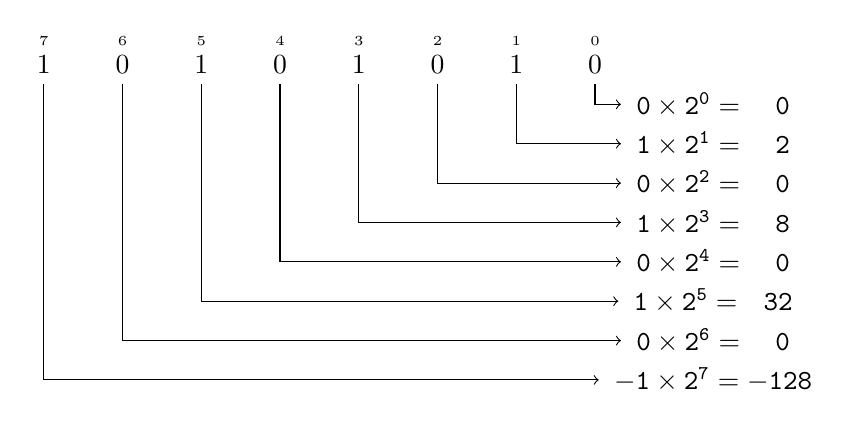
\begin{tikzpicture}[
  flow/.style={draw=black,->,shorten >=2pt}
]
  \node (s7) at (0, 4.3) {\tiny 7};
  \node (s6) at (1, 4.3) {\tiny 6};
  \node (s5) at (2, 4.3) {\tiny 5};
  \node (s4) at (3, 4.3) {\tiny 4};
  \node (s3) at (4, 4.3) {\tiny 3};
  \node (s2) at (5, 4.3) {\tiny 2};
  \node (s1) at (6, 4.3) {\tiny 1};
  \node (s0) at (7, 4.3) {\tiny 0};
  
  \node (n7) at (0, 4) {1};
  \node (n6) at (1, 4) {0};
  \node (n5) at (2, 4) {1};
  \node (n4) at (3, 4) {0};
  \node (n3) at (4, 4) {1};
  \node (n2) at (5, 4) {0};
  \node (n1) at (6, 4) {1};
  \node (n0) at (7, 4) {0};
  
  \node (e7) at (8.5, 0.0) {$\mathtt{-1 \times 2^7 = -128}$};
  \node (e6) at (8.5, 0.5) {$\mathtt{ 0 \times 2^6 = ~~~0}$};
  \node (e5) at (8.5, 1.0) {$\mathtt{ 1 \times 2^5 = ~~32}$};
  \node (e4) at (8.5, 1.5) {$\mathtt{ 0 \times 2^4 = ~~~0}$};
  \node (e3) at (8.5, 2.0) {$\mathtt{ 1 \times 2^3 = ~~~8}$};
  \node (e2) at (8.5, 2.5) {$\mathtt{ 0 \times 2^2 = ~~~0}$};
  \node (e1) at (8.5, 3.0) {$\mathtt{ 1 \times 2^1 = ~~~2}$};
  \node (e0) at (8.5, 3.5) {$\mathtt{ 0 \times 2^0 = ~~~0}$};
  
  \draw[flow] (n7.south) |- (e7.west);
  \draw[flow] (n6.south) |- (e6.west);
  \draw[flow] (n5.south) |- (e5.west);
  \draw[flow] (n4.south) |- (e4.west);
  \draw[flow] (n3.south) |- (e3.west);
  \draw[flow] (n2.south) |- (e2.west);
  \draw[flow] (n1.south) |- (e1.west);
  \draw[flow] (n0.south) |- (e0.west);
\end{tikzpicture}
\end{center}
\end{tcolorbox}
Für die Bits 0 bis 6 ändert sich nichts an der Interpretation, die bereits in Abschnitt \ref{sec:BinaryNumbers} besprochen wurde. Lediglich das Bit 7 wird nun als Vorzeichenbit interpretiert und erhält somit seine \emph{negative Wertigkeit}. Es ergibt sich ein Wert von $-128 + 32 + 8 + 2 = -86$.

\mintinline{c}{int}s sind \emph{vorzeichenbehaftet}. Will man nur positive Zahlen speichern, kann man bei der Deklaration der Variablen den \emph{Modifier} \mintinline{c}{unsigned} benutzen:
\begin{codebox}[Beispiel: Deklaration einer vorzeichenlosen Ganzzahl]
\begin{minted}[linenos]{c}
int main () {
   unsigned int positiv = 9;
}
\end{minted}
\end{codebox}

Was geschieht nun, wenn man einer \mintinline{c}{unsigned}-Variable einen negativen Wert zuweisen will? Betrachten wir das Beispiel:
\begin{codebox}[Beispiel: Zuweisung einer negativen Zahl zu einer unsigned-Variable]
\begin{minted}[linenos]{c}
int main () {
   unsigned char positiv = -1;
}
\end{minted}
\end{codebox}
Hier wird der Compiler zuerst das Bitmuster der Zahl \texttt{-1} mit einer Breite von 8 Bit erzeugen, da ein \mintinline{c}{char} geschrieben werden soll. Dieses Bitmuster lautet \texttt{11111111}. Da die Variable \texttt{positiv} aber ein \mintinline{c}{unsigned char} ist, wird dieses Bitmuster nun als positive Zahl interpretiert und im Folgenden als \texttt{255} gelesen.

Für die Darstellung von Kommazahlen (in der Literatur meist \emph{Fließkommazahlen} genannt) stehen die Datentypen \mintinline{c}{float} (32 bit), \mintinline{c}{double} (64 bit) und \mintinline{c}{long double} (80 bit) zur Verfügung, die im Detail selten verstanden werden müssen. Durch die größere Datenmenge bei \mintinline{c}{double}s und \mintinline{c}{long double}s fallen Rundungsfehler bei der Arbeit mit diesen Typen weniger ins Gewicht, jedoch sind Berechnungen hier zeitaufwändiger. In den meisten Fällen ist \mintinline{c}{double} der am besten geeignetste Datentyp beim Umgang mit Fließkommazahlen.

Es gibt keine vorzeichenlosen Fließkommazahlen.

KursteilnehmerInnen, die sich weiter für den Aufbau von Fließkommawerten interessieren, können nach dem Stichwort \emph{Standard IEEE 754} suchen. Insbesondere finden Sie unter der Adresse \url{https://steve.hollasch.net/cgindex/coding/ieeefloat.html} eine einsteigerfreundliche Erklärung. Im Kurs \emph{Numerik} der Universität Regensburg wird die Darstellung von Fließkommazahlen ebenfalls behandelt.


\subsection{Adressierung -- Pointer} \label{sec:Pointer}
Man kann sich den Arbeitsspeicher als langes Band von kleinen, nummerierten Speicherzellen vorstellen. Jede Zelle fässt genau ein Byte. Um einen Wert zu lesen oder zu schreiben muss dem Prozessor die Nummer der Zelle mitgeteilt werden, die verändert wird. Diese Nummer wird \emph{Adresse} oder \emph{Pointer} genannt. Wenn wir im Code Variablen benutzen, übersetzt der Compiler diese in Adressen. Für die einfachsten Aufgaben kann der Compiler die Speicherverwaltung komplett übernehmen. Wir werden jedoch schon in Kapitel \ref{chp:Input} Situationen kennen lernen, wo wir diese Speicherstruktur kennen müssen. 

\begin{tcolorbox}[title=Speicherbild]
\begin{center}
\begin{tikzpicture}
  [ 
    cell/.style={text width=8mm,
      text height=4mm, draw=black, inner sep=1mm},
    ld/.style={draw=blue,shorten >=2pt,->}
  ]
  \node (c1) at (0,0) [cell] {\ttfamily 99};
  \node (c2) at (1,0) [cell] {\ttfamily 1};
  \node (c3) at (2,0) [cell] {\ttfamily 255};
  \node (c4) at (3,0) [cell] {\ttfamily 0};
  \node (c5) at (4,0) [cell] {\ttfamily 80};
  \node (c6) at (5,0) [cell] {\ttfamily ...};

  \node (labelMem) at (8,  1) {Symbole im Code};
  \node (labelMem) at (8,  0) {Werte im Speicher};
  \node (labelMem) at (8, -1) {Adressen};
  
  \node (a1) [below=2mm of c1]            {\tiny 0x27ff};
  \node (a2) [below=2mm of c2, color=red] {\tiny 0x2800};
  \node (a3) [below=2mm of c3]            {\tiny 0x2801};
  \node (a4) [below=2mm of c4]            {\tiny 0x2802};
  \node (a5) [below=2mm of c5]            {\tiny 0x2803};
  \node (a6) [below=2mm of c6]            {\tiny 0x2804};
  
  \node (ptr) [below=8mm of c1] {\scriptsize Adresse von \texttt{x}};
  \node (vc2) [above=6mm of c1] {\scriptsize Variable \texttt{x}};
  \node (vc0) [above=2mm of c1] {\scriptsize Variable \texttt{y}};
  
  \draw [ld] (ptr.east) .. controls +(0.3,0) .. (a2.south);
  \draw [ld] (vc0.east) .. controls +(0.4,0) .. (c2.north);
  \draw [ld] (vc2.east) .. controls +(2.4,0) .. (c4.north);
\end{tikzpicture}
\end{center}
\end{tcolorbox}

Adressen sind Zahlen und können damit auch im Speicher als binäre Werte abgebildet werden. Abhängig von der \emph{Prozessorarchitektur} handelt es sich dabei um 32bit- oder 64bit-Ganzzahlen. Aus technischen Gründen werden diese meist nicht als \emph{Dezimalzahlen} sondern als \emph{Hexadezimalzahlen} angegeben (\ie mit den \enquote{Ziffern} \texttt{0, 1, 2, 3, 4, 5, 6, 7, 8, 9, A, B, C, D, E, F}. Siehe Abschnitt \ref{sec:NumSystems} für weitere Details hierzu.

Neben der Information, wo im Speicher eine bestimmte Information liegt, muss natürlich auch bekannt sein, wie diese zu interpretieren ist. Daher wird an dieser Stelle zu jedem Datentyp ein zugehöriger \emph{Pointer} eingeführt, also ein Datentyp, der die Adresse einer Information enthält.

Pointer können ebenfalls in Variablen gespeichert werden. Die Deklaration erfolgt wie schon in Abschnitt \ref{sec:DeclareVars}. Der einzige Unterschied ist, dass ein Pointer-Typ gegenüber seinem \emph{Basistyp} durch ein Sternchen \texttt{*} ausgezeichnet wird.

\begin{codebox}[Beispiel: Deklaration von Pointer-Variablen]
\begin{minted}[linenos]{c}
int main () {
   int   normaleVariable;
   int * pointer;
}
\end{minted}
\end{codebox}

Um die Adresse anderer Variablen in Erfahrung zu bringen bedienen wir uns des Adress-Operators \texttt{\&}:

\begin{codebox}[Beispiel: Deklaration von Pointer-Variablen]
\begin{minted}[linenos]{c}
int main () {
   int   normaleVariable;
   int * pointer = &normaleVariable;
}
\end{minted}
\end{codebox}

Wir sagen also, \texttt{pointer} \enquote{zeigt auf} \texttt{normaleVariable}, \ie in der Variablen \texttt{pointer} ist die Information gespeichert, wo \texttt{normaleVariable} im Speicher zu finden ist.

Pointer können \emph{dereferenziert} werden; das heißt, anstatt mit der Adresse selbst zu arbeiten, behandeln wir den Wert, auf den der Pointer zeigt. Dies kann sowohl lesend als auch schreibend stattfinden. Wir benutzen den \emph{Dereferenzierungs-Operator} \texttt{*}:

\begin{codebox}[Beispiel: Dereferenzierung eines Pointers]
\begin{minted}[linenos]{c}
#include <stdio.h>

int main () {
   int   normaleVariable = 5;
   int * pointer = &normaleVariable;
   
   printf("normaleVariable = %d\n", normaleVariable);
   printf("*pointer        = %d\n", *pointer);
   printf("Adresse von normaleVariable: %p\n", pointer);

   *pointer = 8;
   printf("normaleVariable = %d\n", normaleVariable);
}
\end{minted}
\end{codebox}

Wir legen zuerst eine normale Variable mit Wert \texttt{5} an, sowie einen Pointer, der auf diese Variable zeigt. Wenn über den \emph{dereferenzierten Pointer} \texttt{*pointer} in Zeile 8 ein lesender Zugriff stattfindet, passiert genau dasselbe, als würde direkt mit der Variablen \texttt{normaleVariable} selbst gearbeitet werden: \texttt{printf} liest den Wert \texttt{5} aus dem Speicher.
Ebenso ändert auch der Zugriff über \texttt{*pointer} in Zeile 11 tatsächlich den Wert von \texttt{normaleVariable}. Die Ausgabe des Wertes von \texttt{pointer} selbst (also ohne Dereferenzierungs-Operator \texttt{*}) in Zeile 9 liefert eine große Zahl in Hexadezimal-Darstellung, die mit dem \emph{Wert} von \texttt{normaleVariable} nichts zu tun hat.

Folglich lautet die Ausgabe:

\begin{cmdbox}[Ausführungsbeispiel: Dereferenzierung eines Pointers]
\begin{minted}{text}
normaleVariable = 5
*pointer        = 5
Adresse von normaleVariable: 0x7ffdea635c5c
normaleVariable = 8
\end{minted}
\end{cmdbox}

\begin{warnbox}[Große Bedeutung von Pointern in C]
In der Sprache C ist der Umgang mit Pointern unumgänglich. Verinnerlichen Sie daher die soebenen gezeigten Konzepte; wir werden hierauf immer wieder aufbauen.
\end{warnbox}

\FloatBarrier
\begin{figure}
\begin{center}
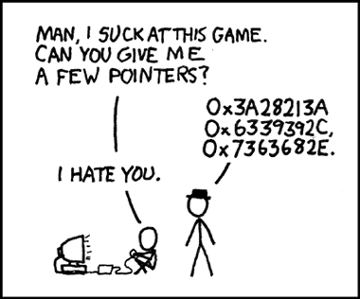
\includegraphics[width=.5\linewidth]{./gfx/xkcd-pointers}
\caption[Pointer im echten Leben]{Pointer im echten Leben. Quelle: \url{https://xkcd.com/138/}}
\end{center}
\end{figure}
\FloatBarrier

\begin{plusbox}
Während C++ ebenfalls Pointer zur Verfügung stellt, die sich dort genauso verhalten wie in der Sprache C, gilt das Paradigma, in C++ \emph{keine} Pointer zu verwenden. C++ kennt andere Konzepte, die Pointer ersetzen (bzw. verstecken) und die helfen, häufige Fehler bei der Arbeit mit Pointern zu vermeiden. Im Rahmen dieses Kurses können leider nur Stichworte genannt werden; sehen Sie dies als Motivation, einen C++-Kurs zu besuchen.

Auch wenn C++-Code \idR keine Verwendung von Pointern macht ist die Kenntnis des Konzepts auch dort sehr wichtig, da der gesamte \enquote{Unterbau} der Sprache auf den hier präsentierten Techniken beruht.
\end{plusbox}

\section{Bitweise Logik und Bit-Shifting} \label{sec:BitwiseOperator}
Für Elektronik-Anwendungen ist es oft nötig, einzelne Schalter an- oder auszuschalten. Meist geschieht dies über eine Zustandsvariable, die an einen \emph{Port} (ein Anschluss, über den Daten fließen können) gesendet wird. Diese Zustandsvariable ist dann \idR eine Ganzzahl-Variable, in der jedes Bit für einen eigenen Schalter steht. Wir benötigen also Mittel, um einzelne Bits zu manipulieren.

Dazu stehen uns die Operatoren \texttt{\~}, \texttt{\&}, \texttt{|}, \texttt{\^}, \texttt{<{}<} und \texttt{>{}>} zur Verfügung.

Die \emph{bitweise Negation} (NOT) \texttt{\~} kehrt jedes Bit um. Betrachten wir die vorzeichenlose 8-Bit-Zahl \texttt{42} (\texttt{00101010}). Das Ergebnis der Negation ist der Wert \texttt{213} (Binärzahl \texttt{11010101}). Als Code lässt sich das wie folgt umsetzen:
\begin{codebox}[Beispiel: Bitweise Negation]
\begin{minted}[linenos]{c}
int main () {
   unsigned char source = 42;
   unsigned char result = ~source;
}
\end{minted}
\end{codebox}

Das \emph{bitweise und} (AND) \texttt{\&} vergleicht die Bits von zwei Werten und setzt das Bit im Ergebnis nur, wenn beide Bits in den Vergleichswerten gesetzt waren (\ie den Wert 1 hatten).

Beim \emph{bitweisen oder} (OR) \texttt{|} werden ebenfalls die Bits von zwei Werten verglichen. Das entsprechende Bit im Ergebnis wird jedoch bereits gesetzt, wenn mindestens eines der Vergleichsbits gesetzt war.

Das \emph{bitweise ausschließliche oder} (XOR) \texttt{\^} arbeitet genauso wie das OR, setzt das Ergebnis-Bit jedoch nur, wenn \emph{genau} eines der Vergleichsbits gesetzt war.

All dies lässt sich in den folgenden Wahrheits-Tabellen ausdrücken:
\begin{codebox}[Wahrheitstabellen: Bitweise Operatoren]
\begin{minted}{text}
     1 1 0 0   12       1 1 0 0   12       1 1 0 0   12
     1 0 1 0   10       1 0 1 0   10       1 0 1 0   10
     - AND -   --       -- OR -   --       - XOR -   --
     1 0 0 0    8       1 1 1 0   14       0 1 1 0    6
\end{minted}
\end{codebox}

Als Code lässt sich das wie folgt umsetzen:
\begin{codebox}[Beispiel: Bitweise Operatoren]
\begin{minted}[linenos]{c}
int main () {
   unsigned char lhs = 12, rhs = 10,
                 and, or, xor;
   and = lhs & rhs;    // =  8
   or  = lhs | rhs;    // = 14
   xor = lhs ^ rhs;    // =  6
}
\end{minted}
\end{codebox}

Die Negation benötigt nur ein \emph{Argument} (Wert, mit dem gearbeitet wird), und wird daher \emph{unärer Operator} genannt. Für AND, OR und XOR sind zwei Werte nötig, weswegen diese als \emph{binäre Operatoren} bezweichnet werden. Die Argumente können auch komplexe Ausdrücke sein, also Ergebnisse von Berechnungen:
\begin{codebox}[Beispiel: Bitweise Operatoren]
\begin{minted}[linenos]{c}
int main () {
   unsigned char result = ~(2 + 7 * (18 & 5));
}
\end{minted}
\end{codebox}

Bitmuster können als ganzes nach links oder rechts verschoben werden. Hierzu dienen die Operatoren \texttt{<{}<} und \texttt{>{}>}.
\begin{codebox}[Beispiel: Bitweise Operatoren]
\begin{minted}[linenos]{c}
int main () {
   unsigned char toLeft  = 170 << 1;
   unsigned char toRight =  85 >> 1;
}
\end{minted}
\end{codebox}
Dies löst folgende Veränderung aus:
\begin{codebox}[Bitshift nach links bzw. nach rechts um jeweils eine Stelle]
\begin{minted}{text}
     1 0 1 0 1 0 1 0   170       0 1 0 1 0 1 0 1    85
     ----- << 1 ----   ---       ----- >> 1 ----   ---
     0 1 0 1 0 1 0 0    84       0 0 1 0 1 0 1 0    42
\end{minted}
\end{codebox}
Bei einem Bitshift nach links werden die Bits am rechten Ende des Bitmusters mit nullen aufgefüllt. Stellen, die am linken Ende über die Registerbreite der aufnehmenden Variable hinaus verschoben werden, gehen verloren. Alles eben gesagte gilt analog für den Bitshift nach rechts.

\begin{hintbox}[Multiplikation mit Zweierpotenzen]
Ein Bitshift um \texttt{n} Stellen nach links entspricht der Multiplikation mit der Zahl $2^{n}$.
Ein Bitshift um \texttt{n} Stellen nach rechts entspricht der Division durch die Zahl $2^{n}$ (Bei Ergebnissen mit Nachkommastelle wird abgerundet). Bitshifts werden schneller durchgeführt als Multiplikationen mit \texttt{*}.

Dies gilt nur für Ganzzahlen, nicht aber für Fließkommazahlen.
\end{hintbox}

\section{Typecasting} \label{sec:Casting}
Es ist gelegentlich notwendig, einen Wert von einem Datentyp in einen anderen umzuwandeln ohne dabei seine Interpretation zu ändern. (Beispielsweise also sollte die Ganzzahl \texttt{3} in die Fließkommazahl \texttt{3.0} umgewandelt werden.) Bei einer solchen Umwandlung ändert sich das Bitmuster, nicht aber der mit diesem Muster dargestellte Wert.

Eine solche Umwandlung wird als \emph{Typecasting} bezeichnet. Die Syntax hierzu ist simpel:
\begin{codebox}[Syntax: Typecasting]
\texttt{(Ziel-Datentyp) Ausdruck}
\end{codebox}
\texttt{Ziel-Datentyp} ist ein beliebiger Datentyp, wie beispielsweise in Anhang \ref{sec:Datatypes} beschrieben. Wie üblich kann \emph{Ausdruck} ein einfacher Wert, eine Variable oder ein komplexer Ausdruck sein.

Ein Grund, den Datentyp zu ändern wurde zum Ende von Abschnitt \ref{sec:OperatorsArithmetic} bereits angeprochen: Operationen wie die Division verhalten sich unterschiedlich, abhängig davon, ob eine Fließkommazahl oder eine Ganzzahl an der Operation beteiligt ist. Solche \emph{Datentyp-spezifischen} Szenarios sind in C sehr häufig.

\begin{codebox}[Beispiel: Typecasting int zu double]
\begin{minted}[linenos]{c}
int main () {
   int x = 7, y = 5;
   double z = (double) x / y;
}
\end{minted}
\end{codebox}

\begin{hintbox}[Reihenfolge der Operationen]
Der Compiler arbeitet \enquote{von links nach rechts}, beachtet aber, dass manche Operationen \enquote{Vorrang} vor anderen haben (\eg Punkt-vor-Strich). Im Obigen Beispiel wird also zuerst der Typecast der Variablen \texttt{x} durchgeführt, und dann der zum \mintinline{c}{double} konvertierte Wert von \texttt{x} durch \texttt{y} geteilt. Damit erhält \texttt{z} den Wert \texttt{1.2}.

Im folgenden Beispiel dagegen erhält \texttt{z} den Wert 1.0:
\begin{codebox}[Beispiel: Fehlerhaftes Typecasting int zu double]
\begin{minted}[linenos]{c}
int main () {
   int x = 7, y = 5;
   double z = (double) (x / y);
}
\end{minted}
\end{codebox}
Durch die Klammern interpretiert der Compiler Zeile 3 als: \enquote{Caste das Ergebnis von \texttt{x / y} zu \mintinline{c}{double}}. Da das Ergebnis von \texttt{x / y} aus der Division zweier \mintinline{c}{int}-Werte hervorgeht, wird hier gerundet und \texttt{z} erhält den (\idR falschen) Wert \texttt{1.0}.
\end{hintbox}

\section{Hierarchie der Operatoren} \label{sec:OperatorHierarchy}
Ausdrücke werden vom Compiler \enquote{von links nach rechts} ausgewertet, wobei die Vorrangigkeit mancher Operatoren beachtet wird. Die Vorrangigkeit kann Tabelle \ref{tab:OperatorPrecedence} im Anhang entnommen werden. Wo immer Unsicherheiten bestehen, kann durch Setzen von (runden Klammern) Sicherheit geschaffen werden.

\section{Zahlenformate -- Hexadezimalsystem} \label{sec:NumSystems}
Gleich zu Beginn dieses Kurses in Abschnitt \ref{sec:BinaryNumbers} haben wir das \emph{Binärsystem} (oder auch \emph{Dualsystem}) kennen gelernt, das neben dem uns vertrauten \emph{Dezimalsystem} steht\footnote{Übrigens: Das Dezimalsystem wäre völlig unbrauchbar, wenn der Mensch nicht zufällig zehn Finger hätte. (Kalenderspruch)}. Nach der dort gezeigten Idee lassen sich Zahlen in beliebigen \emph{Zahlensystemen} bzw. mit beliebiger \emph{Basis} (also Anzahl von verschiedenen Ziffern im Zahlensystem) darstellen. Von besonderer Bedeutung ist das \emph{Hexadezimalsystem} mit 16 Ziffern:

\begin{center}
\texttt{0 1 2 3 4 5 6 7 8 9 A B C D E F}
\end{center}

Um eine Zahl als \emph{hexadezimal} zu kennzeichnen wird häufig der Präfix \texttt{0x} vorangestellt. Der Ausdruck \texttt{0x10} beschreibt also die \emph{Dezimalzahl} 16\footnote{Andere verbreitete Schreibweisen sind \texttt{10h}, \texttt{$10_{16}$} oder \texttt{$10_{hex}$}}. Groß- und Kleinschreibung wird hier nicht unterschieden, es gilt \texttt{0xab} = \texttt{0XAB}.

Die weiteren Informationen in diesem Abschnitt sind für besonders interessierte KursteilnehmerInnen gedacht und müssen für den Kurserfolg nicht im Detail verstanden werden. Sie werden diese Idee aber in der IT-Welt immer wieder antreffen und Nutzen aus dem Verständnis ziehen.

Das Hexadezimalsystem wird immer da verwendet, wo die \emph{Registerbreite} eines Wertes im Speicher Relevanz hat\footnote{Historische Bedeutung hat in diesem Kontext auch noch das \emph{Oktalsystem}, das die Ziffern \texttt{0..7} verwendet. Heute lebt es fast nur noch in dem Witz fort: \emph{Why do programmers confuse Halloween and Christmas? Because Oct 31 = Dec 25...}}. Wir haben bereits gehört, dass ein Computer nur Einheiten zu jeweils 8 Bit behandeln kann. Ein Byte, also eine Gruppe von 8 Bit erlaubt, wie in Abschnitt \ref{sec:Datawidth} erwähnt, 256 verschiedene Werte. Im Hexadezimalsystem wird daraus der \enquote{runde} Wert \texttt{0x100}. Ähnlich ist die Zahl der mit 16 Bit darstellbaren Zahlen gleich \texttt{0x10000} und für 32 bit erhalten wir \texttt{0x100000000} verschiedene Möglichkeiten. Dies ist kein Zufall -- Die Zahl 16 (also die Basis des Hexadezimalsystems) ist eine Potenz der Zahl 2 (also der Basis des Binärsystems). Es besteht eine \enquote{direkte Verwandschaft} zwischen Binärzahlen und Hexadezimalzahlen.

Eine Zahl, die mit $n$ Bit dargestellt wird, kann also mit $\frac{n}{4}$ Hexadezimal-Ziffern geschrieben werden. Dies ist offensichtlich praktischer als lange Ketten von 1en und 0en zu schreiben.

\begin{hintbox}[Farben als Hexadezimal-Werte]
In der Computertechnik werden Farben häufig mit \emph{Hex-Codes} beschrieben. Dies sind sechsstellige Kombinationen aus Ziffern und den Buchstaben A bis F. Tatsächlich sind diese Codes drei aneinander gereihte Hexadezimalzahlen. Diese beschreiben jeweils den Rot-, Grün- und Blau-Anteil einer Farbe. Der Dezimalwert 255 (bzw. die Hexadezimalzahl \texttt{0xFF}) beschreibt dabei \enquote{volle Intensität}, 0 (oder \texttt{0x00} dagegen sagt aus, von der Teilfarbe kommt kein Beitrag. Damit kann die Farbe Orange dann ausgedrückt werden als \texttt{0xFF7F00}: Volle Intensität Rot (\texttt{FF}), halbe Intensität Grün (\texttt{7F}) und Blau-Anteil 0 (\texttt{00}).

Siehe auch \url{https://de.wikipedia.org/wiki/Additive_Farbmischung}
\end{hintbox}

\begin{hintbox}[Zweier-Potenzen in der Computerwelt]
\emph{Alles} in der Computertechnik ist um Potenzen der Zahl 2 aufgebaut. Wir finden 32bit und 64bit-Betriebssysteme, USB-Sticks mit 2, 4, 8 oder 16 GB, oder sogar Bildschirmauflösungen wie 1024x768 Pixel. Diese Zahlen kommen derartig häufig vor, dass sie von TechnikerInnen bereits als \enquote{runde Zahlen} wahrgenommen werden. So feierte beispielsweise Randall Munroe, Author des Webcomics \href{https://www.xkcd.com/}{xkcd} seinen eintausendsten Strip mit dieser Veröffentlichung:

\begin{center}
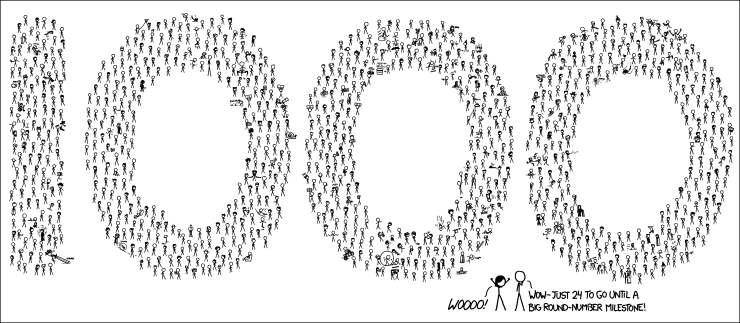
\includegraphics[width=.9\linewidth]{./gfx/xkcd-1000}
\end{center}
\captionof{figure}
	[Dezimale und Binäre runde Zahlen]
	{Dezimale und Binäre runde Zahlen. Quelle: \url{https://www.xkcd.com/1000/}}
\end{hintbox}